\documentclass[a4paper]{article}
\usepackage{amsmath}
\usepackage{bm}
\usepackage{xcolor}
\usepackage{braket}
\usepackage{amssymb}
\usepackage{mathrsfs}
\usepackage{mathtools}
\usepackage{simplewick}
\begin{document}
	\title{chapter\;11}
	\date{ }
	\maketitle
\section{three scattering and non-relativistic correspondence}
\subsection{N+N$\rightarrow$N+N}
The scattering amplitude is$$A_{fi}=-g^2[\frac{1}{(p_1-p_1')^2-m^2+i\epsilon}+\frac{1}{(p_1-p_2')^2-m^2+i\epsilon}]$$
\begin{figure}[htbp]
	\centering
	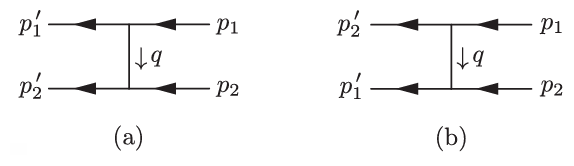
\includegraphics[width=0.6\textwidth]{7.png}
	\caption{N+N$\rightarrow$N+N Feynman diagram}
\end{figure}
In classic case,center-of-momentum frame,this process involves two incoming particles with momentum $\bm{p}_1$ and $\bm{p}_2$ and outgoing particles with momentum $\bm{p}_1'$ and $\bm{p}_2'$.
\begin{figure}[htbp]
	\centering
	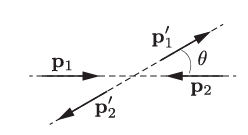
\includegraphics[width=0.6\textwidth]{8.png}
	\caption{classic N+N$\rightarrow$N+N}
\end{figure}

It is convenient to assume that $\bm{p}_1=-\bm{p}_2=|p|\bm{e}$,where $|p|=|\bm{p}_1|=|\bm{p}_2|$.After scattering,the only thing that needs to change is $\bm{e}$ which becomes $\bm{e}'$.Therefore,all 4 momentums can be found to be
\begin{align*}
	&p_1=(\sqrt{|p|^2+\mu^2},|p|\bm{e})\\
	&p_2=(\sqrt{|p|^2+\mu^2},-|p|\bm{e})\\
	&p_1'=(\sqrt{|p|^2+\mu^2},|p|\bm{e}')\\
	&p_2'=(\sqrt{|p|^2+\mu^2},-|p|\bm{e}')\\
\end{align*}
Thus,$(p_1-p_1')^2=-\bm{\Delta}^2$,where $\bm{\Delta}\equiv\bm{p}_1-\bm{p}_1'$,and $(p_1-p_2')^2=-\bm{\Delta}_c^2$,where $\bm{\Delta}_c\equiv\bm{p}_1-\bm{p}_2'$.Therefore,scattering amplitude can be written as$$A_{fi}=g^2[\frac{1}{\bm{\Delta}^2+m^2}+\frac{1}{\bm{\Delta}_c^2+m^2}]$$where $i\epsilon$'s are all dropped as they are useless now.
\par From non-relavitistic perspective$$A_{fiN-R}=\bra{f}V\ket{i}\propto\int d^3\bm{r}V(r)e^{-i\bm{\Delta}\cdot\bm{r}}=\tilde{V}(\bm{\Delta})\propto g^2\frac{1}{\bm{\Delta}^2+m^2}$$if $V(r)=V_{Yukawa}(r)=g^2\frac{e^{-mr}}{r}$.
Now define $exchange\;operator$ $\mathscr{E}$ that exchanges two particles.Consider new potential $V(r)\propto V_{Yukawa}(r)\mathscr{E}$,then$$\bra{f}V\ket{i}=\int d^3\bm{r}V_{Yukawa}(r)e^{-i\bm{\Delta}_c\cdot\bm{r}}\propto g^2\frac{1}{\bm{\Delta}^2_c+m^2}$$
Therefore,the non-relavitistic process of $N+N\rightarrow N+N$ can be viewed as two incoming nucleons scattered by potential $V(r)=V_{Yukawa}(r)(1+\mathscr{E})$ through meson $\phi$.The exchange operator is included as a result of indistinguishability between nucleons.
\subsection{N+$\bar{N}\rightarrow$N+$\bar{N}$}
There are two Feynman diagrams for this process
\begin{figure}[htbp]
	\centering
	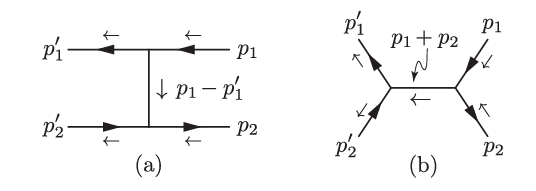
\includegraphics[width=0.6\textwidth]{9.png}
	\caption{N+$\bar{N}\rightarrow$N+$\bar{N}$ Feynman diagram}
\end{figure}

whose scattering amplitude is$$A_{fi}=-g^2[\frac{1}{(p_1-p_1')^2-m^2+i\epsilon}+\frac{1}{(p_1+p_2)^2-m^2+i\epsilon}]$$
As for non-relativistic perspective,the first term in square braket is well understood.While the second term needs to be investigated.Still in center-of-monmentum frame$$p1+p2=(p_1^0+p_2^0,\bm{p}_1+\bm{p}_2)=(E_T,0)$$where $E_T$ is the total energy of two incoming nucleons.Thus the second term in the braket can be written as$\frac{1}{E_T^2-m^2}$.
Recall that in non-relativistic theory,to second order approximation,$$A_{fi}=\bra{f}V\ket{i}+\sum_n\frac{\bra{f}V\ket{n}\bra{n}V\ket{i}}{E_n-E_i}$$This shares similarity with the above expression that they all have poles at $E_i=E_T$ equals some certain energy of energy eigenstate.Therefore,new NR conterpart in process $N+\bar{N}\rightarrow N+\bar{N}$ is pole yielded at energy eigenstate.
\subsection{N+$\phi\rightarrow$N+$\phi$}
There are also two Feynman diagrams for this process.
\begin{figure}[thbp]
	\centering
	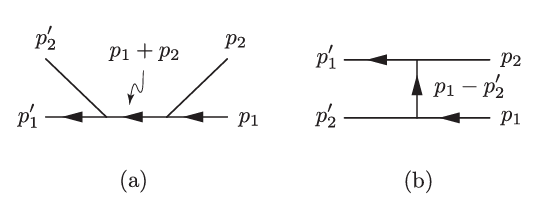
\includegraphics[width=0.6\textwidth]{10.png}
	\caption{N+$\phi\rightarrow$N+$\phi$ Feynman diagram}
\end{figure}

whose scarttering amplitude is$$A_{fi}=-g^2[\frac{1}{(p_1+p_2)^2-\mu^2+i\epsilon}+\frac{1}{(p_1-p_2')^2-\mu^2+i\epsilon}]$$
which is identical to case 2 except that the mass term in the denominator is $\mu$,the mass of nucleon,instead of $m$,the mass of meson.In center-of-monmentum frame,four-momenta are
\begin{align*}
	&p_1=(\sqrt{|p|^2+\mu^2},|p|\bm{e}),for\;nucleon\\
	&p_2=(\sqrt{|p|^2+m^2},-|p|\bm{e}),for\;meson\\
	&p_1'=(\sqrt{|p|^2+\mu^2},|p|\bm{e}')\\
	&p_2'=(\sqrt{|p|^2+m^2},-|p|\bm{e}')\\
\end{align*}
Therefore,
$$(p_1-p_2')^2=(\sqrt{|p|^2+\mu^2}-\sqrt{|p|^2+m^2})^2-\bm{\Delta}_c^2$$
Now.the first term in the square braket in scarttering amplitude is still associated to pole at energy eigenstate,the second term however,is associated with something else.The denominator of second term can be written as $$\frac{1}{\bm{\Delta}^2_c+\mu^2-(\sqrt{|p|^2+\mu^2}-\sqrt{|p|^2+m^2})^2}$$
It is believed that this term can be associated with some Yukawa potential with range R and $$\frac{1}{R^2}=\mu^2-(\sqrt{|p|^2+\mu^2}-\sqrt{|p|^2+m^2})^2$$which is dependent of energy of incoming nucleon and meson.
\par Therefore,the NR picture for this term is meson and nucleon interact via an energy dependent Yukawa potential.
\section{crossing symmetry}
Yukawa potential,exchange Yukawa potential and energy eigenstate pole are actually different aspects of one same thing.This can be viewed as some symmetry called crossing symmetry.(different from Noether symmetry which is associated with conservative quantity.)
\par Consider the most general 4 particles system.Let 4 inward lines represent 4 types of particles equipped with its own momentum.
\begin{figure}[htbp]
	\centering
	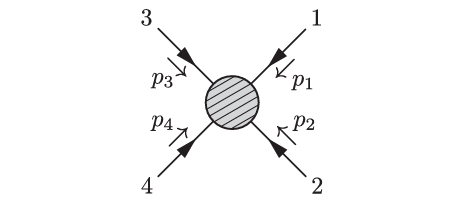
\includegraphics[width=0.6\textwidth]{11.png}
	\caption{4 particles system}
\end{figure}

This diagram can be read from 3 directions and each direction is corresponding to one physical process.
\begin{align*}
	(i)&1+2\rightarrow\bar{3}+\bar{4}\quad(right\quad to\quad left)\\
	(ii)&1+3\rightarrow\bar{2}+\bar{4}\quad(top\quad to\quad down)\\
	(iii)&1+4\rightarrow\bar{2}+\bar{3}\quad(swapping\quad1\quad and\quad2\quad then\quad right\quad to\quad left)
\end{align*}
Of course,there are other three process,but they can be found via CPT transformation of above three.There are some rules for this diagram
\par (1)momenta conservation:$p_1+p_2+p_3+p_4=0$
\par (2)positive energy(zeroth component of p) corresponds to incoming particle and negative energy corresponds to outgoing particle.
\par To describe scattering,only two parameters are needed,energy and scattering angle.Now,however,define three quantities
\begin{align*}
	&s=(p_1+p_2)^2=(p_3+p_4)^2\\
	&t=(p_1+p_3)^2=(p_2+p_4)^2\\
	&s=(p_1+p_4)^2=(p_2+p_3)^2
\end{align*}
One and only one of these 3 quantities is conserved in one pariticular scattering process out of three mentioned above.If this process conserves s,then call it s-channel process and so on for t,u.
\par there is constraint on $s,t,u$ and it is easily check that$$s+t+u=\sum_im_i^2$$where $m_i$ is mass of particle $i^{th}$.Therefore,variables $s,t,u$ are lying on a plane.
\begin{figure}[htbp]
	\centering
	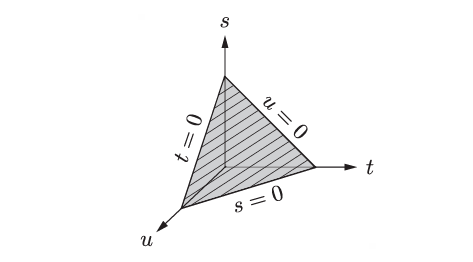
\includegraphics[width=0.6\textwidth]{12.png}
	\caption{(s,t,u) lie on plane s+t+u=$\sum_im_i^2$}
\end{figure}

Now call these variables Mandelstam variables.In this plane,define 3 unit vectors $\hat{\bm{e}}_s,\hat{\bm{e}}_t,\hat{\bm{e}}_u$ that are perpendicular to contour lines of 3 variables.Directions are pointing inward the shadow zone.
\begin{figure}[htbp]
	\centering
	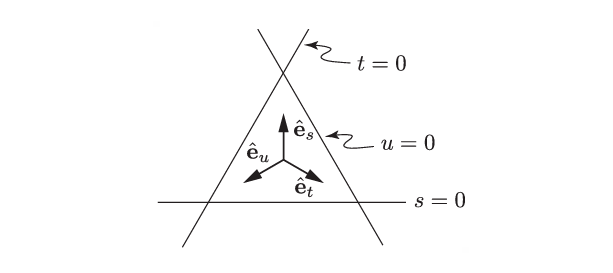
\includegraphics[width=0.6\textwidth]{13.png}
	\caption{3 unit vectors}
\end{figure}
\vspace{0.05\textheight}
\par It is clear that,in this plane,and for any vector $\bm{r}$ in this plane
\vspace{0.05\textheight}
\begin{align*}
	&\hat{\bm{e}}_s+\hat{\bm{e}}_t+\hat{\bm{e}}_u=0\\
	&\bm{r}=\frac{2}{3}(s\hat{\bm{e}}_s+t\hat{\bm{e}_t}+u\hat{\bm{e}_u})
\end{align*}

\vspace{0.1\textheight}
where $s,t,u$ are directed distance from piont $\bm{r}$ to corresponding base line of these 3 variables.
\begin{figure}[htbp]
	\centering
	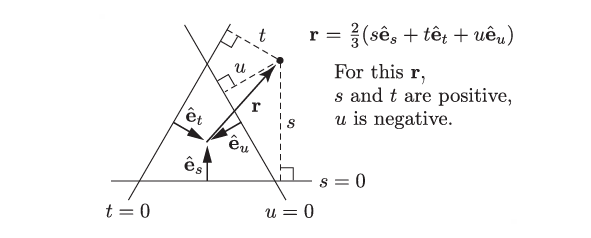
\includegraphics[width=0.6\textwidth]{14.png}
	\caption{s,t,u for $\bm{r}$}
\end{figure}

Note that given a point,namely a set of (s,t,u),it does not have to correspond to a real physical process.The threshold and region of a,say,s-channel process can be complex,if the particles are quite different.
\end{document}